\section{서론}

개인의 성취는 노력, 환경, 그리고 운이 복합적으로 작용하여 결정된다.\footnote{본 연구는 \citet{onj17}의 연구에 노동패널의 최신 자료를 판올림한 글이다.} 존 롤즈(\citeauthor{Rawls99})는 동일한 천부적 능력과 야망을 가진 사람들이 그 사람의 가정환경, 상속된 부의 크기, 인종, 성 등과 무관하게 동등한 성취의 전망(prospects of success)을 가질 때 ``공정한 기회평등''이 보장된다고 하였다.\footcite[p. 63.]{Rawls99} 이러한 롤즈의 입장은 드워킨(\citeauthor{dworkin81a}), 아네슨(\citeauthor{arneson91}), 코헨(\citeauthor{cohen89}), 로머(\citeauthor{Roemer98}) 등에 의하여 평등주의의 대표적인 분배 원칙으로 자리 잡게 되었다.\footnote{\citet{dworkin81a, dworkin81b}, \citet{arneson91}, \citet{cohen89}, \citet{Roemer98}}

노력에 따라 발생하는 불평등에 대해서는 마땅히 그 개인이 책임져야 하겠지만 개인의 의지와 무관하게 주어지는 환경에 따라 발생하는 불평등에 대해서까지 개인에게 책임을 지워서는 안 된다는 것이 본 논문의 전체에 일관된 기회평등에 대한 기본 입장이다. \footcite[p.5.]{Roemer98} 즉, 개인에게 도덕적 책임이 없는 환경이 성취에 미치는 영향은 모든 사람들에게 중립적으로 작용하여야 하고, 따라서 더 이로운 환경도 더 불리한 환경도 없도록 해야 한다는 것이다. 이러한 기회평등의 기본 정신에 대해서는 상당히 높은 수준의 사회적 합의가 있으며 복지선진국들이 추구하는 사회정책의 기본 방향이기도 하다.

기회불평등한 사회에서는 개인의 의지나 선택과 관계없이 타고난 사회$\cdot$경제적 환경이 그 사람의 성취 전망의 우열을 결정하게 된다. \citet{letl08, letl09}은 환경 별로 얻어진 성취(소득) 분포들 간의 ``확률지배관계''가 존재할 경우 기회불평등이 존재한다고 정의하고 미국과 유럽의 주요 국 소득자료를 통하여 소득기회불평등의 존재와 크기를 분석하였다. 본 연구의 주된 목적은 이러한 \citeauthor{letl08}의 실증적 방법론을 활용하여 우리나라의 소득 기회불평등의 존재와 크기를 분석하고 선행연구와 비교하는 것이다.

급속한 경제성장에도 불구하고, 우리나라의 소득불평등은 1990년대 초반기 낮은 수준을 유지해 왔었고 세대 간 계층 상승의 기회도 비교적 높은 수준이었던 것으로 알려져 있다. 이러한 고성장-저불평등의 구조는 1990년대 중반이후 흐려지기 시작하여, 2000년을 지나 현재에 이르기까지 소득불평등은 빠른 속도로 악화되었다. 높은 불평등과 양극화를 겪으면서 기회평등에 대한 국민들의 신뢰는 크게 약화되었고 자녀 교육을 통한 신분상승의 희망도 사라지고 있다.

이러한 주관적 인식의 급격한 변화와 달리 세대 간 계층이동에 대한 여러 선행연구들은 비교적 낙관적인 결론을 보였다. 본 연구와 동일한 한국노동패널 자료를 이용한 \citet{cnh11}과 \citet{yang12}은 세대 간 소득탄력성(부모소득상승률에 대한 자녀소득 상승률의 비율)을 0.37이하로 추정하여 OECD국가 평균 이하었다. 이는 우리나라의 세대 간 계층이동성이 OECD 평균 보다 높은 것을 의미한다. \footnote{선행연구인 \citet{kim09}과 \citet{ketl09} 등에서는 이보다 더 낮은 탄력성이 보고되기도 하였다.} 따라서 적어도 세대 간 소득탄력성의 기준으로 볼 때 우리나라의 기회불평등은 비교적 낮은 수준이라는 것이다.

이렇게 한국노동패널 자료 분석에서 나타난 결과가 앞서 인용된 통계청 「사회조사」의 결과와 차이가 나는 이유로는, 우선 자료에 반영된 성인들의 대부분이 1990년대 중반 이전에 초중고 교육을 받은 세대에 속하는 점을 들 수 있다. 이 세대에서 교육을 통한 계층상승의 기회가 비교적 공평하게 주어졌다는 주지의 사실에 비추어 볼 때 높은 세대 간 계층이동성은 자연스러운 결과라 할 수 있다. 둘째로, 설문조사에 나타난 세대 간 계층이동에 대한 주관적 인식이 세대 간 소득탄력성 만으로 나타내기 어려운 기회불평등의 양상들을 반영한 결과일 수 있다는 점이다. 가령, 눈에 띄게 변화한 대학진학에 있어서 소득계층 및 지역 간 격차와 계층 사다리로서의 교육의 역할이 약해진 점 등을 들 수 있다.

\citet{knl08}은 기회불평등을 최소화하는 세율과 실제 세율을 비교하는 방식(\citet{retl03})을 적용하여 우리나라의 기회불평등도가 OECD국가들 중에서 미국과 이탈리아처럼 높은 나라에 속함을 보인 바 있다.
이처럼 세대 간 소득 탄력성만으로는 포착하기 어려운 기회불평등의 다차원적 연구를 통하여 소득 계층이동에 대한 주관적 인식 변화에 대한 합당한 설명을 제시할 수 있는 가능성은 열려 있다고 볼 수 있다.  
본 연구와 동일한 방법을 활용하여 교육적 성취(대학입학 수학능력평가 성적)의 기회불평등을 연구한 \citet{ohetl16}에서는 우리사회에 교육성취의 기회불평등이 뚜렷하게 나타남을 보여주고 있다.
더 이상 우리사회에서 교육의 계층사다리 기능이 작동하기 어렵다는 이러한 결과는 앞서 소개된 통계청 조사를 잘 설명한다고 볼 수 있다.
교육 자료는 어린 청소년들을 대상으로 하여 성인을 대상으로 하는 소득 자료 보다 세대 간 계층이동성에 대한 주관적 인식 변화의 흐름을 더 잘 반영한다고 볼 수 있다.
 본 연 구에서는 선행연구들에서 사용한 한국노동패널의 가구소득자료를 기초로 \citet{letl08, letl09}에 소개된 기회불평등의 존재와 크기에 대하여 살펴 볼 것이다.
 
 만일 A라는 환경에 놓인 사람이 B라는 환경에 놓인 사람보다, 동일한 노력을 할 때 항상 더 높은 성취의 가능성을 갖는다면 두 사람에게 보장된 성취의 기회가 평등하다고 볼 수 없고 A에게 더 우월한 성취의 기회가 보장된다고 말할 수 있다.
 어떤 두 환경 사이에도 이처럼 하나가 다른 하나보다 더 우월한 성취의 기회를 보장한다고 할 수 없을 때 기회평등이 달성되는 것이다.
 이러한 기회평등 개념에 기초하여 \citet{letl08, letl09}은 미국, 이탈리아, 노르웨이, 스웨덴 등의 주요 선진국에서 부모 학력별 (혹은 직업별) 소득분포들을 도출하고 이들 간에 우열관계의 유무를 검증하는 방식으로 기회평등의 유무를 확인하였다.

본 연구에서는 \citeauthor{letl08}과 동일하게 가구주의 학력과 직업이라는 두 가지 환경변수를 활용하여 상이한 환경 간의 기회불평등의 존재 여부를 살펴보았다.
 분석 결과 두 환경 변수 모두에 있어서 소득 성취의 기회불평등이 존재하는 것으로 나타났다.
 \citet{letl08, letl09}에서 얻어진 결과와 비교할 때, 우리나라의 기회불평등은 비교적 기회불평등이 뚜렷한 미국, 프랑스, 이태리와 유사하게 나타나고 기회불평등이 존재하지 않거나 그 정도가 낮은 스웨덴, 노르웨이, 독일과는 다르게 나타났다.
 또한 개천용기회불평등지수(최상위소득계층에서의 최하위환경비율)를 이용한 분석에서 2000년대 초반 이후로 기회불평등도가 다소 상승하는 경향이 있다는 사실을 확인할 수 있었다(개천용지수는 본 연구와 동시에 진행된 교육기회불평등에 대한 연구, \citet{ohetl16}에서도 소개된 바 있다).
 
기회평등의 원칙은 \citet{Roemer98}와 \citet{letl08, letl09}에 의하여 실증 모형에 도입되었고 경험적 분석에 활용될 수 있게 되었다.
 \citet{letl08}은 프랑스 소득자료를 바탕으로 부모의 직업을 환경변수로 하여 총 여섯 개의 서로 다른 집단간에 기회불평등이 존재하는지 여부를 검증하여 기회의 불평등이 존재함을 보였다.
 \citet{letl09}는 동일한 연구방법을 유럽각지의 8개국과 미국을 대상으로 실시하여 스웨덴, 노르웨이 같은 북유럽 국가의 경우 기회평등한 사회임을 보였다.
 
기회불평등에 대한 국내 선행연구로 \citet{knl08}와 \citet{knl11}은 아버지의 학력과 직업이 자식의 소득획득 기회에 중요한 영향을 미친다는 사실을 밝힌 바 있다.
 또한 아버지의 학력, 성별, 출생년도, 성장기 지역, 형제자매 수 등의 여러 환경요인들을 고려한 \citet{jnl16}의 최근 연구에서도 소득불평등에서 환경이 차지하는 비중이 매우 높다는 것이 확인되었다.

\section{모형과 기본개념}
개인의 소득은 개인의 노력뿐만 아니라 개인의 선택과 무관하게 주어지는 사회경제적 환경(부모의 경제력과 학력), 선천적인 재능, 그리고 여러 우연적 요인들에 의하여 결정된다.
노력의 차이가 발생시킨 소득 격차는 일정 부분 용인되어야 하겠지만 사회경제적 환경의 차이가 야기하는 불평등까지 용인할 수 없다는 것이 본 연구의 기본적인 전제이다.

환경 $c$와 노력 $e$가 다른 우연적인 요인들과 결합되어 만들어내는 소득 $y$의 조건부 확률분포를 $y=F(y|c)$라 하자. 
\footnote{본 연구의 기본모형은 소득 기회 불평등에 대한 연구인 \citet{letl08, letl09}의 모형을 따르고 있다.}
즉 임의의 두 환경 에 대해 가 성립한다는 의미이다.
가장 강한 형태의 기회평등의 원칙은, 임의의 두 환경 $c,c' \in C$에 대하여 각 노력수준 에서 결정되는 수능성적의 분포가 동일해야 한다는 조건 $F(\cdot | c) = F(\cdot | c')$으로 정의할 수 있다. 
하지만 이러한 기회평등은 과도하게 이상적이라 할 수 있고, 본 연구에서는 이를 완화한 \citet{letl08, letl09}의 기회평등 개념을 활용한다. 
\citeauthor{letl08}의 두 논문이 실증모형, 기본개념 그리고 이론적 정리들을 자세히 소개하고 있으나 완결성을 위하여 핵심적인 내용들을 본 절에서 간략히 다시 정리할 것이다.

\subsection{기회불평등}
 
 상이한 두 환경 $c$와 $c'$에서 개인의 노력 $e$는 각각 $F(\cdot |c,e)$와 $F(\cdot |c',e)$의 소득 전망을 제공한다고 볼 수 있다. 
만약 모든 노력수준 $e$와 모든 소득수준 $y$에서
\begin{equation}
    F(x | c) \leq F(x | c')
    \label{eq:klips_fdom}
\end{equation}
이 성립하면 환경 $c'$에서서 노력 수준에 무관하게 항상 일정소득 $y$를 초과하는 소득을 획득하는데 실패할 확률이 환경 $c$에서 보다 크거나 같다는 것을 의미한다.
이는 소득획득의 전망의 관점에서 환경 $c'$이 환경 $c$보다 열악하다는 것이다.
이처럼 적어도 두 개의 환경 $c,c'$에서 식 (\ref{eq:klips_fdom})이 성립하고 적어도 하나의 소득수준에서 이 부등식이 강부등식으로 성립하여 두 환경사이에 제 1차 확률지배관계가 형성되는 경우에 제1차 기회불평등이 존재한다고 정의한다.

식 (\ref{eq:klips_fdom})의 제1차 확률지배관계를 제2차 확률지배관계로 대체하여, 모든 노력수준 $e$와 모든 소득수준 $x$ 에서,
\begin{equation}
   \int_{0}^{x} F(y | c)\,dy \leq \int_{0}^{x} F(y | c')\,dy
    \label{eq:klips_sdom}
\end{equation}
의 관계가 성립하고 적어도 하나의 $x$에서 강부등호 관계가 성립하는 두 개의 환경 $c,c' \in C$이 존재할 때 제2차 기회불평등이 존재한다고 정의한다. 

제1차(제2차) 기회평등은 이와 같이 제1차(제2차) 기회불평등이 존재하지 않을 때 성립한다.
\footnote{\citet{letl09}에서 EOP-W1, EOP-W2 참고.} 
 기회평등이 성립하더라도 상이한 두 환경에서 얻어지는 성취의 확률분포들이 동일할 필요가 없을 뿐만 아니라 두 환경 중 하나에서 성취의 기댓값의 더 큰 것도 허용된다.
 또한 모든 노력 수준에서 확률지배관계가 성립해야 기회불평등이 존재하는 것으로 정의하고 있어서 적어도 한 노력 수준에서만 확률지배관계가 없다면 기회평등이 성립하게 된다. 
 이처럼 본 연구에서 정의하는 기회평등은 최소한의 원칙이라는 점에 주목할 필요가 있다.
 
두 환경 사이에 식 (\ref{eq:klips_fdom})과 같은 기회불평등이 존재하면, 어떤 효용함수를 상정하더라도 환경 $c$의 소득분포 $F(\cdot |c,e)$에서 기대효용이 환경 $c'$의 소득분포 $F(\cdot |c,e)$에서 보다 더 클 것이다.
  즉, 항상 환경 $c$가 $c'$ 보다 선호될 것이다.
  소득에 대하여 위험기피적인 선호를 가정하면, 두 환경 사이에 식 (\ref{eq:klips_sdom})와 같은 기회불평등이 존재할 때도 항상 환경 $c$가 $c'$ 보다 더 큰 기대효용 가져 선호될 것이다.
  
만일 노력 수준 그 자체가 환경에 영향을 받는다면 앞에서 정의한 기회불평등 개념은 기회불평등의 기본원리를 적절히 담고 있다고 볼 수 없을 것이다.
 가령 환경 $c$가 환경 $c'$ 보다 노력하기 용이한 환경이라고 하자.
 각 노력에서 소득의 확률분포가 두 환경에서 동일하더라도 (따라서 앞서 정의에 따라 기회평등이 성립하는 경우) 환경 $c$에서 노력하는 것이 더 용이하다면, 결과적으로 환경 $c$가 환경 $c'$ 에서 보다 소득획득에 유리한 환경이 된다.
 따라서 이 경우 기회평등이 보장되었다고 보기 힘들 것이다.
 환경으로 야기되는 불평등을 개인의 책임으로 돌리지 않아야 한다는 기회평등의 기본 원리에 따르자면 개인의 노력도 환경의 영향이 배재된 순수한 노력을 기준으로 해야 한다는 것이 \citet{Roemer98}의 주장이다.
 따라서 본 연구에서는 \citet{letl08, letl09}에서와 같이 환경에 영향을 받지 않는 순수한 노력을 고려할 것이다.
  
순수한 노력을 고려할 때 앞에서 정의된 기회불평등은 훨씬 단순한 조건으로 나타낼 수 있다.
 환경에 무관하게 균일한 분포를 가지는 노력을 가정하면, 제1차와 제2차 기회불평등에 대한 아래의 필요조건을 각각 얻을 수 있다.
\footnote{이에 대한 보다 자세한 논의는 \citet{letl09} Proposition 4 참고.}

제1차 기회불평등조건: 어떤 두 환경 $c$, $c'$에 대하여 $F(\cdot |c)$와 $F(\cdot |c')$사이에 제1차 확률지배관계가 성립한다.
 
제2차 기회불평등조건: 어떤 두 환경 $c$, $c'$에 대하여 $F(\cdot |c)$와 $F(\cdot |c')$사이에 제2차 확률지배관계가 성립한다.
 
이하에서는 이 두 조건에 나타난 확률지배관계 검증 중심으로 실증분석이 이루어진다.
검증은 \citet{dnd00}의 비모수 검증법이 이용될 것이다.
먼저 환경을 기준으로 집단을 나누고 집단별 혹은 환경별 소득분포 $F(\cdot |c)$를 얻는다.
이렇게 얻어진 환경별 분포함수들 간에 확률지배 여부를 검증한다.
확률지배 검증을 통하여 분포 $F(\cdot |c)$가 $F(\cdot |c')$을 1차(2차) 확률 지배를 하나 그 역은 성립하지 않을 시 전자가 후자를 1차(2차) 확률지배하는 것으로 확인된다.
만약 두 분포가 서로 확률지배 관계가 확인되지 않을 경우 두 분포의 일치여부를 검증할 것이다.
  
\subsection{기회불평등 지수}
기회불평등의 유무뿐만 아니라 기회불평등 지수를 이용하면 기회평등의 크기를 측정하고 이를 활용하여 시점 또는 국가 간 비교가 가능하다. 
\citet{letl08}에서 사용된 기회불평등지수를 정의하기 위하여, 환경 $t$의 평균소득을 $\mu _t$ , 불평등도(지니계수)를  $G _t$로 나타내고 환경 의 ``가치''를 $\mu _t (1-G _t)$로 나타낸다. 평균소득이 클수록 그리고 불평등도가 낮을수록 환경의 가치는 높아지는 것을 알 수 있다. 모든 환경에 대하여 이렇게 환경의 가치를 측정하고 이러한 가치 값들에 대한 불평등도를 지니계수로 구한 것이 지니(Gini) 기회불평등지수(이하, GO 지수)이다. 총 $k$개의 환경이 있고 환경 가치의 평균값을 $\mu$라고 하면, 각 환경 $t$의 비중이 $P_t$일 때, 지니 기회불평등지수는 다음과 같이 주어진다.
확률지배검증은 기회불평등의 존재 유무만을 알려준다.
그러나 똑같이 기회불평등한 사회 간에도 기회불평등의 크기를 비교하려면 기회불평등 지수가 필요하다.
\begin{equation}
    G O=\frac{1}{\mu} \sum_{i=1}^{k} \sum_{j>i} P_{i} P_{j}\left(\mu_{j}\left(1-G_{j}\right)-\mu_{i}\left(1-G_{i}\right)\right).
    \label{eq:klips_GOI}
\end{equation}

열악한 환경에서도 최상위 성취전망이 높은 사회에서는 계층상승의 기회가 크다고 할 수 있다.
이처럼 최하위에서 최상위로의 계층상승의 전망을 반영하는 지표도 기회불평등지표로 유용하게 활용될 수 있다.
 가장 열악한 환경 $\underline{c}$에 처한 사람들의 전체인구에서의 비율을  $q_{\underline{c}}$이라 하자.
 최상위 성취 집단을 소득 상위 $p$퍼센트에 속하는 사람들이라고 하고 이들의 수를 $n_p$라고 하자.
 그리고 이들 중 가장 열악한 환경  $\underline{c}$에 처한 사람들의 수를  $n_{p,\underline{c}}$라고 하면, 개천용(기회)불평등지수(이하, RR 지수)는 최상위 성취집단에서 최하위 환경의 비율을 이용하여 다음과 같이 정의된다.
\footnote{개천용지수는 본 연구와 동시에 진행된 교육기회불평등에 대한 연구인 \citet{ohetl16}에서 소개된 바 있다.}
\begin{equation}
    R R_{p}=1-\frac{n_{p, \underline{c}} / n_{p}}{q_{\underline{\underline{c}}}} .
    \label{eq:klips_RRI}
\end{equation}
 

개천용불평등지수 값이 0이라는 것은 최상위 성취를 이룬 사람들 중에서 최하위 환경을 가진 사람들의 비율이 최하위 환경 사람들의 인구비율과 동일하다는 것을 의미하고 이는 기회불평등이 없는 상태를 나타낸다.
개천용불평등지수 값이 1이라는 것은 반대로 최상위 성취를 이룬 사람들 중에서 최하위 환경을 가진 사람이 없다는 것을 의미하고 이는 기회불평등도가 가장 높은 상태를 나타낸다.
개천용불평등지수 값이 음이 되는 경우도 있는데 이는 최하위 환경이 최상위 성취를 달성하는데 오히려 유리한 ``역''기회불평등의 상태를 말한다.

개천용불평등지수가 0인 사회에서는 가장 열악한 환경에서도 다른 환경과 동일한 확률로 성공이 보장된다고 볼 수 있다.
개천용불평등지수가 양수 의 값을 가진다면 최악의 환경에서 성공할 수 있는 100명 중에서 $100 \times q$명(퍼센트)가 기회불평등 때문에 성공하지 못하는 것으로 볼 수 있다.
예를 들어 개천용불평등지수가 0.6인 사회에서는 최악의 환경에서 성공할 수 있는 100명중에서 60명이 기회불평등 때문에 실패하게 되는 것이다.

\section{자료 및 변수}

본 연구에서 사용할 자료는 한국노동패널(Korean Labor and Income Panel Study, KLIPS) 제1차에서 제22차 자료이다.
KLIPS 자료는 1998년부터 도시에 거주하는 한국의 5,000 가구와 그 가구원을 대상으로 시작한 매년 1회 조사하는 종단연구다.
2009년에 1,415가구 그리고 2018년에 5,044가구를 표본에 추가하였는데 이는 표본이탈로 인한 대표성 감소와 농촌과 같은 도시 가구 이외의 가구를 포함하여 전국적 대표성을 확보하기 위함이다.
가장 최신인 22년차(2019년) 자료는 전국의 12,000여 가구의 구성원 23,000 여명을 대상으로 조사가 진행되었다.
본 연구는 1998-1999년, 2004-2003년, 2011-2012년, 그리고 2018-2019년, 네 개의 시기를 중심으로 결과를 소개하고 나머지 시기에 대한 분석결과는 부록으로 제시한다.

분석의 대상인 성취는 분석 대상 가구주의 가계 총소득으로 한다.
가계 총소득은 한 해 동안 가계에서 획득한 근로소득, 금융소득, 부동산소득, 사회보장 및 이전소득 등을 합한 가처분소득이다.
가구구성원 수에 따른 소득의 규모 차이는 가구구성원 총수의 제곱근을 나누어 균등화하였다.
98년 조사가 97년의 소득에 관하여 묻는 점을 감안하여 한국은행에서 발표하는 한 해 전의 물가지수를 반영한다.
그리고 \citet{letl08}의 결과인 외국사례와 비교 편의를 위해 각 연도 모든 가구의 소득은 해당연도 가구 소득의 평균으로 나눈 값을 이용하였다.
마지막으로 매해 발생하는 우발적 소득의 영향을 줄이기 위하여 앞서 방식으로 구한 소득의 2개년 평균을 사용한다.
설문에 응답하지 않은 연도의 소득은 인접한 연도의 소득과 같다고 가정했다.
\footnote{예를 들어 1, 2, 3년의 소득이 각각 1만 원, 무응답, 5천 원일 경우 1, 2년의 평균소득은 1만 원이고 2, 3년의 평균소득은 5천 원이다.}
그리고 \citet{letl08}의 선행연구와 비교에 용이하도록 각 년도 가구의 소득은 해당년도 가구소득의 평균으로 나눈 값으로 나타냈다.

사회경제적 환경변수로 소득획득에 영향을 주는 주요 요인인 가구주 부친의 교육수준과 가구주 부친의 직업(가구주 14세 무렵의 부친 직업) 두 가지를 선정하였다.
먼저 교육수준은 중졸 이하를 저학력, 고교재학 또는 졸업을 중학력, 초대졸 입학 이상을 고학력으로 하는 세 가지 수준으로 분류하였다.
직업 수준은 한국직업표준분류상 농림어업 종사자를 저숙련, 사무·서비스·판매업·단순 노무 종사자를 중숙련, 의회 의원·고위임직원 및 관리자·전문가·기술공과 준전문가를 고숙련으로 범주화하였다.

초중등 교육의 급속한 팽창에서 발생하는 편의(bias)를 최소화하면서 \citet{letl08}과의 비교를 위하여 매 조사년도에 30세 이상 50세 이하에 해당하는 가구주들에 대하여 별도의 분석을 진행 하였다.
이 연령구간은 \citet{letl08}의 분석에서 사용된 자료의 연령대(25-40세 혹은 25-50세 자료)와 비슷할 뿐만 아니라, \citeauthor{letl08}의 경우 연령대를 변화시키더라도 큰 차이가 없었으므로, 해당 연령구간에서 적절한 상호비교가 가능하다.
우리나라의 경우 연령대의 변화가 연구 결과에 큰 영향을 주는데 이는 연령대별로 부모 학력 분포에 급격한 차이가 발생하기 때문이다.
특히 연령대가 높아질수록 저학력 부모를 가진 사람들의 비율이 급격히 높아지고, 동시에 초중고 교육의 급속한 팽창의 시기에 성장한 사람들의 비율이 높아진다.
따라서 이러한 편의를 피하고 동시에 우리나라의 청년실업이 상대적으로 높고 입대와 문화적 특성으로 사회진출이 늦다는 점을 고려할 때 가장 적절한 비교 가능 연령집단을 30-50세로 보았다.
 
\begin{table}[htbp]
    \centering
    \resizebox{\textwidth}{!}{
\begin{tabular}{c|c|r|r|c|c|r|r|c|c}
\hline \multirow{2}{*}{년도} & \multirow{2}{*}{환경수준} & \multicolumn{4}{c|}{ 가구주 부친 직업 환경 } & \multicolumn{4}{c}{ 가구주 부친 교육수준 환경 } \\
\cline { 3 - 10 } & &  자료수  & 환경내비중 & 평균 & 분산 & 자료수 & 환경내비중 & 평균 & 분산 \\
\hline \multirow{3}{*}{1998 (1차)} & 저 & 1626 & $63.01\%$ & $0.9484$ & $0.7940$ & 1681 & $62.49\%$ & $0.9451$ & $0.7489$ \\
\cline { 2 - 10 } & 중 & 632 & $24.40\%$ & $1.0786$ & $0.8466$ & 622 & $22.87\%$ & $1.1214$ & $1.0084$ \\
\cline { 2 - 10 } & 고 & 164 & $6.19\%$ & $1.3242$ & $1.0876$ & 224 & $7.91\%$ & $1.3780$ & $1.2183$ \\
\hline \multirow{3}{*}{2004 (7차)} & 저 & 1276 & $58.44\%$ & $0.9674$ & $0.7117$ & 1284 & $55.61\%$ & $0.9400$ & $0.7083$ \\
\cline { 2 - 10 } & 중 & 697 & $31.65\%$ & $1.0542$ & $0.8487$ & 763 & $32.55\%$ & $1.1153$ & $0.8514$ \\
\cline { 2 - 10 } & 고 & 147 & $6.51\%$ & $1.1574$ & $0.6962$ & 199 & $8.41\%$ & $1.2285$ & $0.9034$ \\
\hline \multirow{3}{*}{2011 (14차)} & 저 & 1131 & $45.18\%$ & $0.9902$ & $0.5657$ & 1128 & $41.49\%$ & $0.9649$ & $0.5482$ \\
\cline { 2 - 10 } & 중 & 1063 & $42.38\%$ & $1.0756$ & $0.6027$ & 1249 & $45.66\%$ & $1.0812$ & $0.6078$ \\
\cline { 2 - 10 } & 고 & 234 & $9.10\%$ & $1.1992$ & $0.8321$ & 262 & $9.54\%$ & $1.2573$ & $0.8514$ \\
\hline \multirow{3}{*}{2017 (20차)} & 저 & 802 & $32.91\%$ & $0.9897$ & $0.6420$ & 774 & $29.33\%$ & $0.9742$ & $0.6185$ \\
\cline { 2 - 10 } & 중 & 1283 & $52.27\%$ & $1.0334$ & $0.6095$ & 1470 & $55.26\%$ & $1.0347$ & $0.5907$ \\
\cline { 2 - 10 } & 고 & 270 & $10.87\%$ & $1.2016$ & $0.8067$ & 313 & $11.53\%$ & $1.2225$ & $0.8494$ \\
\hline
\end{tabular}
}
    \caption{분석 자료의 기초통계량}
    \label{tab:klips_stat_selected}
\end{table}

 30-50세로 가구주 연령대를 제한하더라도, 조사 첫해인 1998년 저학력환경 가구의 비율은 62.40\%로 그해 가장 큰 집단이었으나 꾸준히 감소하여 마지막 조사년도에는 35.06\%까지 줄었고 중학력 환경이 53.36\%로 가장 큰 비중을 차지하게 된다.
 이와 같은 양상은 직업 환경에서도 나타난다.
 전체 연령대를 고려할 경우 베이비붐 세대의 은퇴로 인해 소득이 낮은 고연령층에서 저수준의 비율이 해가 갈수록 급속히 증가하게 되어 저수준 집단의 낮은 소득에 연령효과가 더해진다.
 이로 인하여 기회불평등도는 더 커지게 되고 조사 기간 동안 증가하는 양상을 뚜렷이 보이게 된다.
 
\section{환경별 기회불평등의 분석}

각각의 환경에 대한 분석 결과는 다음의 순서로 진행된다.
 먼저 환경 유형별 분포의 형태를 살펴보고 이들 분포에 대한 확률지배검증을 통해 기회불평등 존재 여부를 살펴본다.
 다음으로 지니기회불평등지수와 개천용불평등지수를 조사 기간 전년도에 걸쳐 측정함으로써 기회불평등도의 변화 추이를 살펴본다.

\subsection{가구주 부친 직업 환경}
 가구주 부친의 직업에 따라 환경유형별 집단의 누적분포와 확률밀도를 구한 결과는 그림 (\ref{fig:klips_cdf4_byedu})와 그림 (\ref{fig:klips_pdf4_byedu})과 같다. 앞서 표 (\ref{tab:klips_stat_selected})에서 본 것과 같이 모든 년도에서 환경수준이 좋아질수록 평균적인 성취가 더 높은 것을 알 수 있다. 
 
\begin{figure}[htbp]
    \centering
    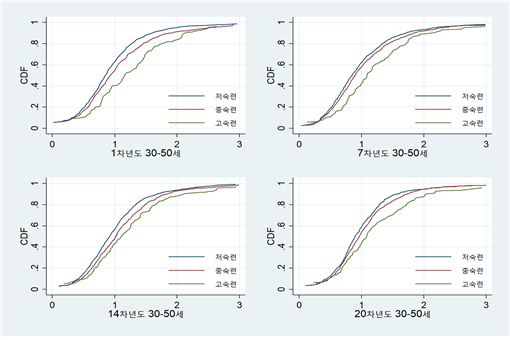
\includegraphics[scale=.7]{figure/klips_cdf4_byedu.png}
    \caption{가구소득의 누적분포: 가구주부친직업환경, 가구주연령 30-50세}
    \label{fig:klips_cdf4_byedu}
\end{figure}

각 년도의 누적분포는 환경수준이 높을수록 왼쪽에 위치하여 분명한 확률지배관계가 존재하는 것으로 보인다.
하지만 왼쪽 끝에 위치한 소득이 매우 낮은 가구들의 누적분포에서 환경수준 간 교차가 일어나는 것을 볼 수 있다.
따라서 모든 소득수준을 대상으로 하는 확률지배검증의 특성상 상이한 환경간의 확률지배가 없다는 결과를 도출할 가능성이 높다.
이러한 경향을 통제하기 위해 각 환경수준별 최하위 5 퍼센트와 최상위 5퍼센트를 제외한 가운데 90 퍼센트의 자료만으로 확률지배검증을 실시하였다.
 
\begin{figure}
    \centering
    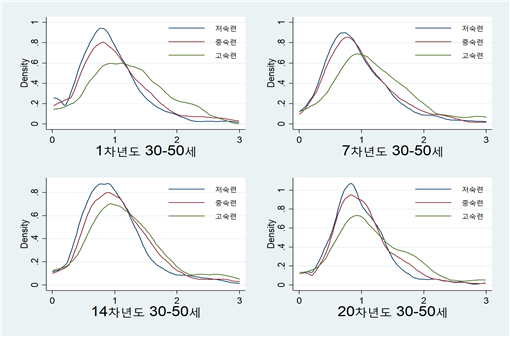
\includegraphics[scale=.7]{figure/klips_pdf4_byedu.png}
    \caption{가구소득의 확률분포: 가구주부친직업환경, 가구주연령 30-50세}
    \label{fig:klips_pdf4_byedu}
\end{figure}

매 조사년도에 연령이 가구주 연령이 30-50세인 가구들을 대상으로 확률지배 검증을 통해 기회불평등의 유무를 살펴보았다.
\footnote{모든 조사년도에 대한 확률지배 검증결과는 부록에 제시한다.}
그 결과 조사기간 전체에서 다수의 환경유형 쌍에서 확률지배관계가 존재하는 것으로 나타났다.
표 (\ref{tab:klips_dom_byjob})에 요약된 4개년도의 경우 총 12개의 환경유형 쌍 가운데 5개에서 확률지배 관계가 존재하는 것으로 나타났다.
1차년도와 20차년도에서 고숙련 집단이 다른 두 수준의 집단 모두를 확률지배 하여 기회불평등이 존재하였다.
전체년도로 확장하여 살펴보더라도 저숙련 집단과 중숙련 집단간에는 기회불평등이 존재하는 년도가 22개 년도 가운데 네 개 년도에 불과하지만 고숙련이 경우는 10이상의 조사년도에서 저숙련 집단이나 중숙련 집단에 대하여 2차 확률지배를 하여 기회불평등이 존재하는 것으로 나타난다.
그러나 다수의 열악한 환경이 우월한 환경을 확률지배 하는 경우는 전혀 없었다.

\begin{table}[htbp]
    \centering
    \caption{가구소득 누적분포의 확률지배 검증결과: 가구주부친직업환경, 가구주연령 30-50세}
    \resizebox{\textwidth}{!}{
\begin{tabular}{c|cc|cc|cc|cc}
    \hline \multirow{2}{*}{환경유형} & \multicolumn{2}{c|}{1차년도(1998)} & \multicolumn{2}{c}{7차년도(2004)} & \multicolumn{2}{|c|}{14차년도(2011)} & \multicolumn{2}{c}{20차년도(2017)} \\
    \cline{2-9} & 중숙련 & 고숙련 & 중숙련 & 고숙련 & 중숙련 & 고숙련  & 중숙련 & 고숙련  \\
    \hline 저숙련 & ? & $<_2^{***}$ & $<_2^{*}$  & ? & $<_2^{**}$  & ?  & ? & $<_2^{***}$ \\
    중숙련 & - & $<_2^{***}$ & - & ?  & - & ? & - & $<_2^{***}$ \\
    \hline
\end{tabular}}
    \confer{집단별 상하위 5\%를 각각 제외하고 검증. $=$ 은 동일한 확률분포, $<_{1}$은 행이 열에 1차 확률지배, $<_{2}$는 행이 열에 2차 확률지배 당하는 관계,  $?$는 확률지배관계를 확인 불가능한 경우임. ($*: \alpha = 0.5, **: \alpha = 0.01, ***: \alpha = 0.001$.)}
    \label{tab:klips_dom_byjob}
\end{table}

기회불평등 지수를 이용하여 연도별 기회불평등도의 추이를 분석한 결과는 그림 (\ref{fig:klips_jobgrp})와 같다.
먼저 기회불평등 전체의 추세를 알 수 있는 지니기회불평등지수부터 살펴본다.
가구주 연령을 30-50세로 제한 할 경우 전연령에 대상으로 하는 경우에 비하여 기회불평등 정도가 낮은 수준임을 알 수 있다.
반면 기회불평등 지수의 년도별 변동은 가구주 연령을 30-50세로 제한한 경우가 큰 것을 알 수 있다.
이는 앞서 언급한 바와 같이 연령을 통제하지 않은 경우에 환경변수의 비중이 변하면서 저수준집단이 고령화에 의한 소득감소의 효과를 받고, 고령자들은 은퇴이후 소득의 변동이 거의 없기 때문이다.
가구주 연령의 제한이 없는 경우  1998년부터 2006년까지는 기회불평등이 0.026 근처를 유지하는 모습을 보인다.
2007년부터 불평등 지수가 급상승 하여 2008년 이후는 평균 약 0.03의 수치를 보여 전후가 확연히 다른 모습을 보인다.
2017년부터 불평등 지수가 또 한번 가파른 상승을 하는네, 두 해 모두 노동패널 자료의 보충이 있었던 시기라는 공통점이 있다.

가구주의 연령을 30-50세로 제한하는 경우, 같은 기간동안 기회불평등도는 2007년 전후를 제외하고 0.02-0.026 사이에서 등락을 거듭하는 모습을 보인다.
COVID-19의 충격을 받은 2020년의 가구소득이 반영된 22회차에서 기회불평등 지수가 하락하는 모습을 보였다.
 
\begin{figure}
    \centering
    \caption{기회불평등지수 추이: 가구주부친직업환경}
    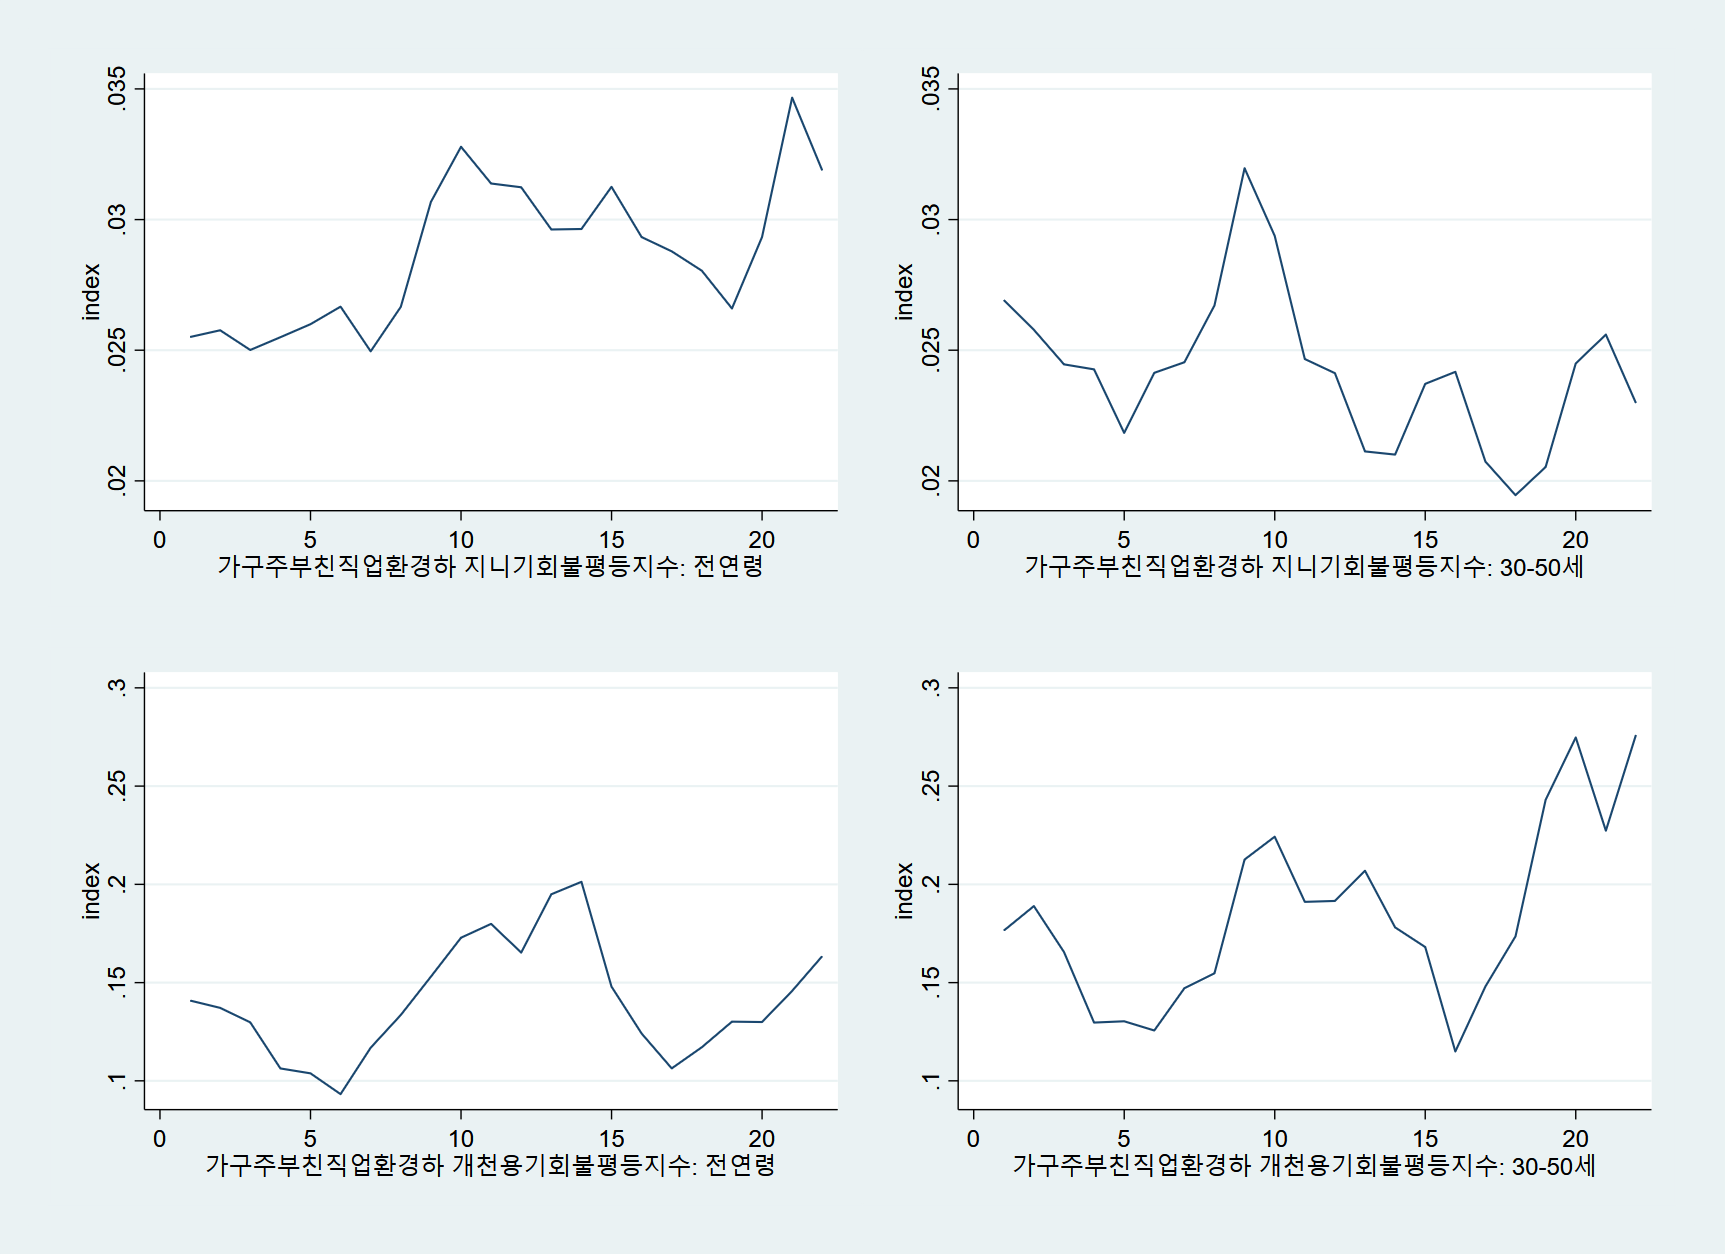
\includegraphics[width=\textwidth]{figure/incn1m_jobgrp_index.png}
    \label{fig:klips_jobgrp}
\end{figure}

개천용지수로 봤을 때 전연령과 30-50대의 기회불평등은 앞서와는 다른 모습이다.
가구주 연령을 제한하는 경우가 전연령을 대상으로 하는 경우보다 개천용 지수가 높게 나타나서 전반적인 기회불평등과 성공의 기회불평등이 상이함을 보이고 있다.
반면 연령대를 30-50으로 제한하는 경우 앞서와 마찬가지로 지수의 년도별 변동폭은 커짐을 알 수 있다.
특히 17차년인 2015년 이후부터 30-50세의 지수값과 전연령에서의 지수값의 격차가 크게 벌어지고 있다.
2020년 소득이 반영된 22회차 지수는 지니기회불평등 지수와는 다르게 전년도보다 상승하는 모습을 보였다.
우리 사회에서 체감하는 기회불평등에 대한 세대별 인식의 차이는 특히 소득상위 20\%와 같이 높은 수준의 성취를 대상으로 할 때 발생할 수 있음을 시사한다.

\subsection{가구주 부친 학력 환경}

가구주 부친의 교육 환경에 따라 얻어진 누적분포함수와 확률밀도함수를 각각 <그림 \ref{fig:klips_cdf4_byjob}>와 <그림 \ref{fig:klips_pdf4_byjob}>에 정리하였다.
가구주 부친의 직업을 환경변수로 했던 앞서의 결과와 마찬가지로 학력수준이 높은 집단일수록 누적분포가 아래에 위치하고 확률밀도가 오른쪽으로 치우치는 것을 볼 수 있다.

\begin{figure}
    \centering
    \caption{가구소득의 누적분포: 가구주부친직업환경, 가구주연령 30-50세}
    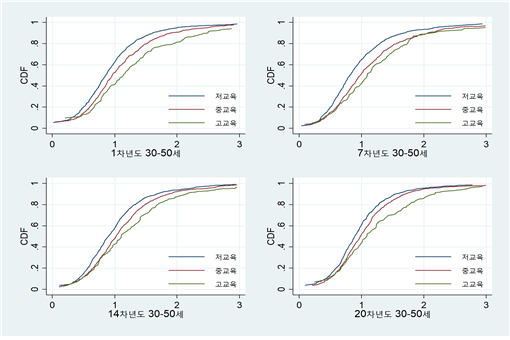
\includegraphics[scale=.7]{figure/klips_cdf4_byjob.png}
    \label{fig:klips_cdf4_byjob}
\end{figure}

\begin{figure}
    \centering
    \caption{가구소득의 확률분포: 가구주부친직업환경, 가구주연령 30-50세}
    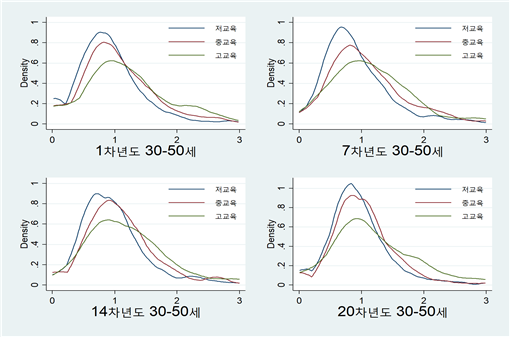
\includegraphics[scale=.7]{figure/klips_pdf4_byjob.png}
    \label{fig:klips_pdf4_byjob}
\end{figure}

확률지배 검증결과는 <표 \ref{tab:klips_dom_byedu}>과 같다.
4개의 조사년도 모두에서 고교육에 의한 저교육의 확률지배가 있어 특정집단간에 꾸준한 기회불평등이 있음을 알 수 있다.
학력환경하에서도 고교육 집단은 다른 집단들에게 확률지배 당하는 경우가 없어 기회불평등한 상황에 놓이지 않았다.
중교육집단 역시 저교육 집단에게 기회불평등한 년도는 없었다.

\begin{table}[htbp]
    \centering
    \caption{가구소득 누적분포의 확률지배 검증결과: 가구주부친학력환경, 가구주연령 30-50세}
    \resizebox{\textwidth}{!}{
\begin{tabular}{c|cc|cc|cc|cc}
    \hline & \multicolumn{2}{|c|}{1차년도(1998)} & \multicolumn{2}{c}{7차년도(2004)} & \multicolumn{2}{|c|}{14차년도(2011)} & \multicolumn{2}{c}{20차년도(2017)} \\
    \hline 환경수준 & 중교육 & 고교육 & 중교육 & 고교육 & 중교육 & 고교육  & 중교육 & 고교육  \\
    \hline 저교육 & ? & $<_2^{***}$ & $<_2^{**}$ & $<_2^{***}$ & $<_2^{*}$ & $<_2^{***}$ & $<_2^{**}$ & $<_2^{***}$ \\
    중교육 & - & $<_2^{**}$ & - & ?  & - & ? & - & ? \\
    \hline
\end{tabular}}
    \confer{집단별 상하위 5\%를 각각 제외하고 검증. $=$ 은 동일한 확률분포, $<_{1}$은 행이 열에 1차 확률지배, $<_{2}$는 행이 열에 2차 확률지배 당하는 관계,  $?$는 확률지배관계를 확인 불가능한 경우임. ($*: \alpha = 0.5, **: \alpha = 0.01, ***: \alpha = 0.001$.)}
    \label{tab:klips_dom_byedu}
\end{table}

지수를 이용한 가구주부친학력환경하 기회불평등의 추이는 <그림 \ref{fig:klips_edugrp}> 과 같다.
먼저 지니기회불평등지수를 앞서의 직업환경하에서 도출한 수치들과 비교한다.
가구주 부친의 학력을 환경으로 하는 경우 직업을 환경으로 하는 경우보다 0.005 높은 기회불평등 수치를 보이고 있다.

전연령의 경우 직업환경하에서 나타났던 2007년경의 기회불평등 상승 추세는 관찰되지 않는다. 
하지만 2016년의 기회불평등 상승은 앞서와 같은 양상이지만 더 높은 수치로 나타나고 있다.
30-50세 집단은 5차년도인 2002년 부터 2016년 까지 기회불평등이 꾸준히 감소하는 모습을 보이지만 여전히 직업환경 하의 수치들 보다는 높다.

\begin{figure}
    \centering
    \caption{기회불평등지수 추이: 가구주부친학력환경}
    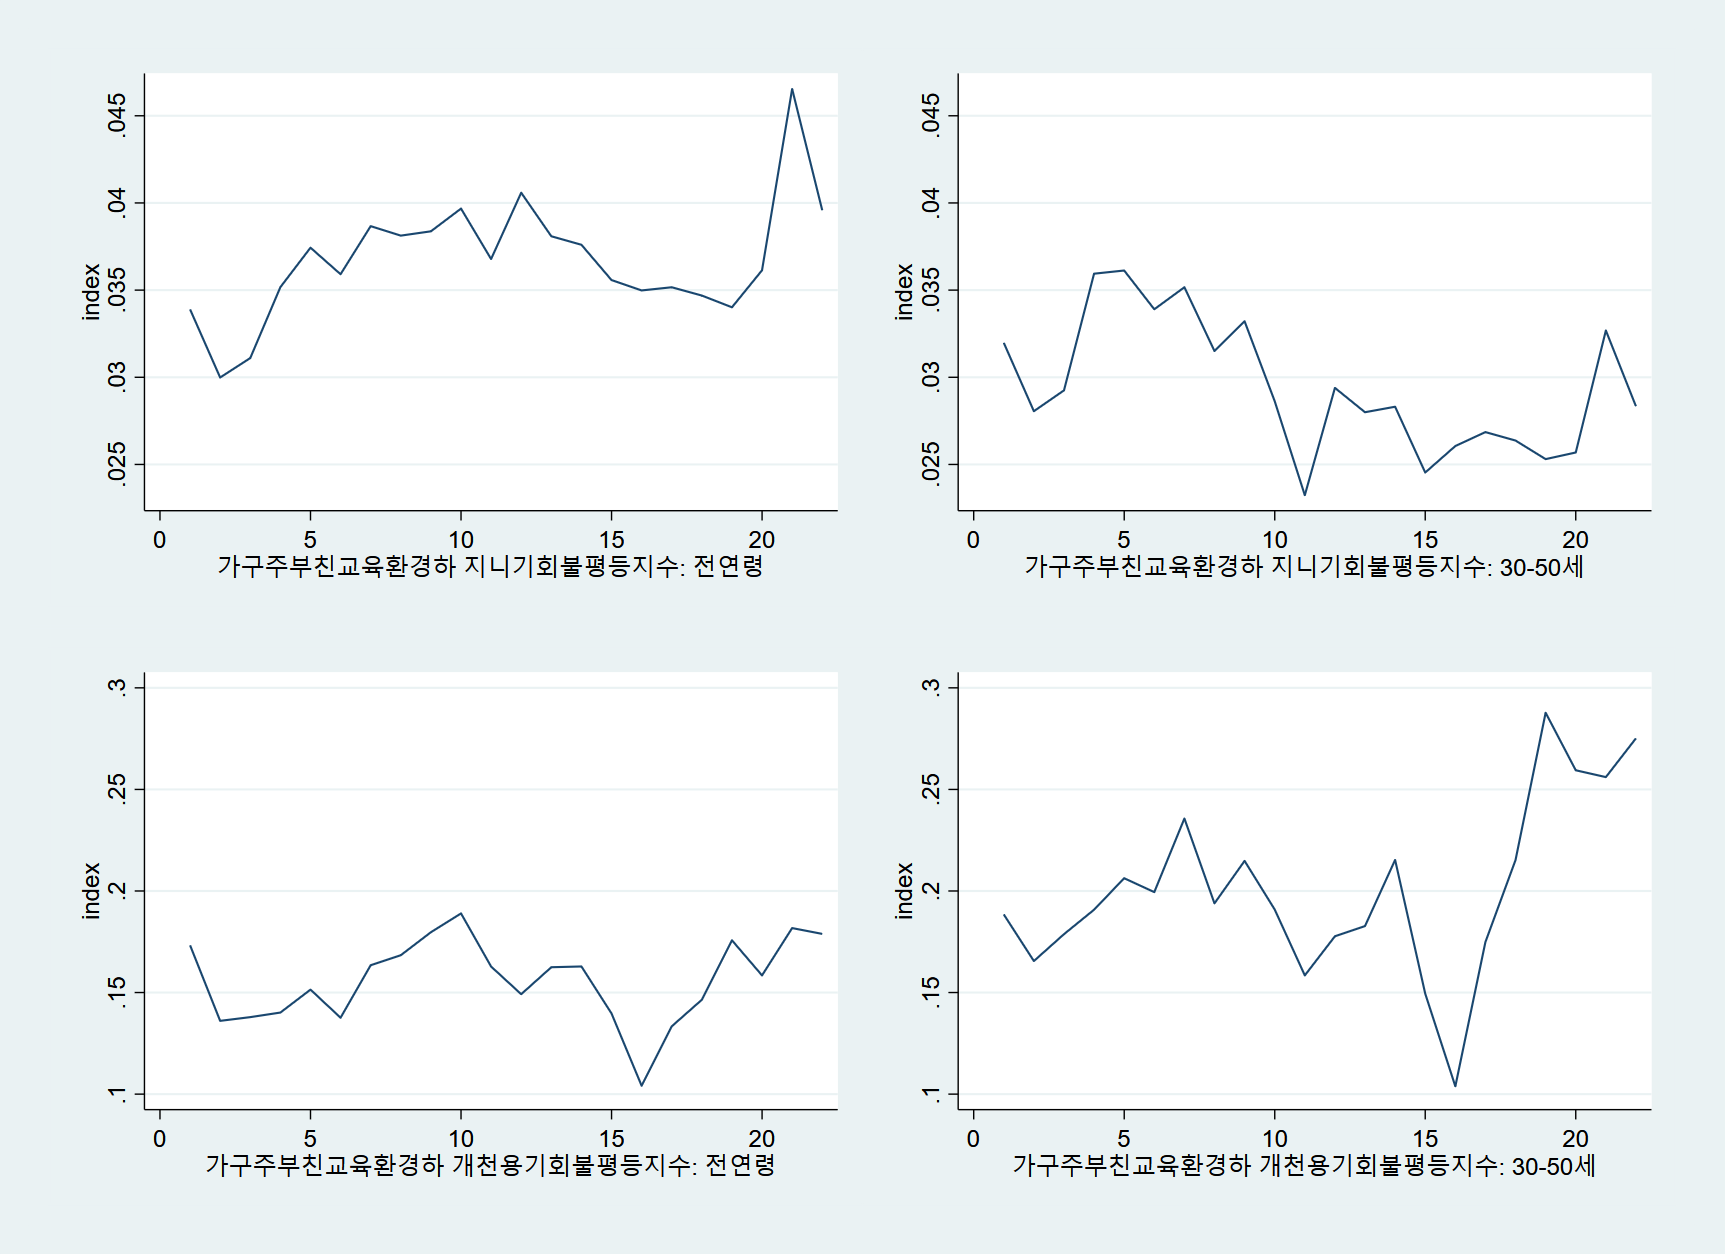
\includegraphics[width=\textwidth]{figure/incn1m_edugrp_index.png}
    \label{fig:klips_edugrp}
\end{figure}

개천용기회불평등지수의 경우 지니기회불평등지수와는 다르게 직업환경과 학력환경에서 지수값 차이가 거의 없다.
30-50세 집단의 경우 17년차인 2015년 이후 기회불평등 수치의 급격한 상승을 보이고 있다.
이 추세는 앞선 직업환경하에서 나타나는 모습과 동일하여 지니기회불평등 지수의 추세가 가구주 연령의 제한여부에 따라 다른 양상을 보이는 것과 구분된다.

\section{미국과 유럽 연구결과와의 비교}

\citet{letl08}는 90년대 초반 유럽 전역의 8개국과 미국의 소득자료를 이용하여 가구주 부친의 학력을 환경변수로 하여 세 가지 환경수준으로 구분하고 확률지배검증을 통한 기회불평등 존재유무 검증과 지니기회불평등지수 계산을 수행하였다.
 그 가운데 일부 내용을 소개하여 한국과 비교하고자 한다.
 
\begin{figure}
    \centering
    \caption{스웨덴, 노르웨이, 이탈리아, 미국의 가계소득 누적분포: 가구주부친 학력환경}
    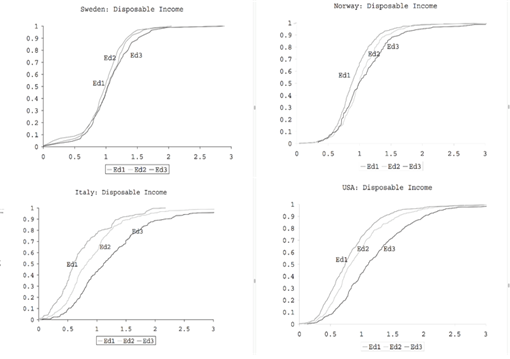
\includegraphics[width=\textwidth]{figure/letl08.png}
    \source{\citet{letl08}}
    \confer{Ed1: 저교육, Ed2: 중교육, Ed3: 고교육.}
    \label{fig:letl08}
\end{figure}

<그림 \ref{fig:letl08}>은 스웨덴, 노르웨이, 이탈리아, 미국 4개국의 1990년대 초·중반에 측정된 가구주 부친의 학력을 환경변수로 한 환경수준별 누적밀도분포이다.
 먼저 위 열의 두 그림과 아래 열의 두 그림이 확연한 차이를 보이는 것을 알 수 있다.
 스웨덴의 경우 환경수준별 누적분포의 간격이 거의 없이 일치하는 것을 볼 수 있고, 노르웨이도 중학력(Ed2)과 고학력(Ed3) 집단간의 누적분포가 거의 차이가 없는 것을 알 수 있다.
 반면, 아래의 이탈리아와 미국은 <그림 5>에서 한국의 1998년 경우보다 환경수준별 누적밀도분포의 간격이 더 큰 것을 알 수 있다.

이러한 결과는 확률지배검증의 결과로도 확인되는데 스웨덴은 놀랍게도 가처분소득 기준으로 기회평등을 달성한 것으로 나온다.
 반면 이탈리아와 미국의 경우는 모든 환경수준의 쌍에서 2차 확률지배관계가 있는 것으로 나오는데 분포의 양 끝 5\% 제외한 우리의 검증결과에 대입해 보면 모두 1차 확률지배관계로 나올 것으로 생각할 수 있다.
 
 \begin{table}[htbp]
     \centering
     \caption{국가별 지니기회불평등지수 비교}
     \begin{tabular}{c|c|c|c}
\hline 국가 & 자료년도 & 지수값 & 표준편차 \\
\hline 한국$^{*}$ & 1998 & $3.19$ & $0.780$ \\
\hline 스웨덴$^{***}$ & 1991 & $1.09$ & $0.606$ \\
\hline 노르웨이$^{***}$ & 1995 & $2.18$ & $0.581$ \\
\hline 이탈리아$^{***}$ & 1993 & $7.64$ & $0.531$ \\
\hline 미국$^{***}$ & 1991 & $6.93$ & $0.586$ \\
\hline 독일$(서독)^{**}$ & 1994 & $0.88$ & $0.426$ \\
\hline 영국$^{***}$ & 1991 & $3.45$ & $0.683$ \\
\hline 프랑스$^{*}$ & 1994 & $4.22$ & $0.406$ \\
\hline 벨기에$^{***}$ & 1992 & $4.58$ & $0.581$ \\
\hline
\end{tabular}
     \\
     \source{한국을 제외한 수치는 \citet{letl08}.}
     \confer{가구주연령대는 *:30-50세, **:25-45세,  ***25-50세.}
     \label{tab:klips_letl08}
 \end{table}

표 \ref{tab:klips_letl08} 는 한국과 \citet{letl08}에서 계산된 지니기회불평등지수의 값을 나열한 자료이다. 스웨덴, 노르웨이의 지수 값은 각각 1.09와 2.18로 이탈리아 미국의 7.64와 6.93에 비해 훨씬 낮은 수치이다. 비록 한국의 자료조사연도가 나머지 국가에 비해 늦기 때문에 비슷한 시점에서의 비교라고 할 수는 없겠지만 그 정도는 영국, 프랑스 벨기에 등과 비슷하며 이탈리아, 미국보다는 기회불평등 정도가 낮은 것으로 나온다.

\section{소결론 및 시사점}
가구주의 환경별로 가구들의 가처분소득 확률분포를 도출하고 이러한 분포들 사이의 확률지배관계로 정의되는 기회불평등의 유무를 검증하고 기회불평등도를 분석하였다.
 가구주 부친의 직업과 학력이라는 두 가지 환경변수를 활용하여 기회불평등의 존재 여부를 살펴본바, 두 환경 모두에서 기회불평등이 존재하는 것으로 나타났고 가장 높은 수준의 환경집단은 나머지 집단을 거의 모든 경우에 확률지배하는 것을 알 수 있었다.
 
지니기회불평등지수와 개천용 지수를 이용한 기회불평등도를 분석한 바, 학력을 환경변수로 사용하는 경우가 직업을 사용하는 경우에 비해 기회불평등도가 더 큰 것을 알 수 있었다.
 지니 기회불평등지수의 경우 가구주의 연령대를 제한할 경우 제한하지 않을 때보다 불평등 정도가 크게 내려갔다.
 이는 과거 빠른 경제성장의 효과로 인한 교육기회의 양적 증가와 산업구조의 고도화 결과 우리가 환경으로 생각하는 변수들이 크게 변했고, 따라서 은퇴 등으로 인해 소득이 많이 감소하는 고연령층일수록 열악한 환경에 처한 가구의 비중이 크기 때문이다.
 또한, 나이를 제한하는 경우 지수값이 일정한 추세를 나타내는 것 역시 환경의 변동을 나이 제한으로 통제한 결과로 볼 수 있다.
 가구주의 나이를 30-50세로 제한한 경우 최근 년의 개천용지수가 급상승하는데 이는 우리 사회가 체감하는 높은 기회불평등은 주요경제활동연령층이 경제적 성공을 얻는 데 대한 기회불평등임을 보여주고 있다.

향후 연구과제는 다음과 같다.
먼저 기회불평등을 없애는데 필요한 최소한의 부의 이전을 생각해 볼 수 있다.
우리의 연구방법에서 기회불평등은 확률지배검증의 결과인데 그렇다면 확룰지배가 일어나지 않게 누적분포가 서로 교차할 수 있게 하는 환경수준 간 피구-달튼 형태의 소득 이전을 하나의 예시로 생각해볼 수 있다.
이를 통해 기회불평등 해소를 위한 최소한의 재분배정책의 규모를 가늠해볼 수 있다.
다음으로 경제위기가 기회불평등에 주는 영향에 대하 알아볼 필요성이 제기된다.
COVID-19로 시작된 경제위기가 우리 사회의 소득의 기회불평등에 어떤 영향을 주는지에 대한 구체적인 연구가 진행되어야 할 것이다. 현재는 2020년 한 해의 소득자료만 관찰 가능 하지만 자료가 추가되는 2-3년 이내에 구체적인 연구가 가능할 것으로 생각된다.